\chapter{Spanning trees}

\index{spanning tree}

A \key{spanning tree} of a graph consists of
all nodes of the graph and some of the
edges of the graph so that there is a path
between any two nodes.
Like trees in general, spanning trees are
connected and acyclic.
Usually there are several ways to construct a spanning tree.

For example, consider the following graph:
\begin{center}
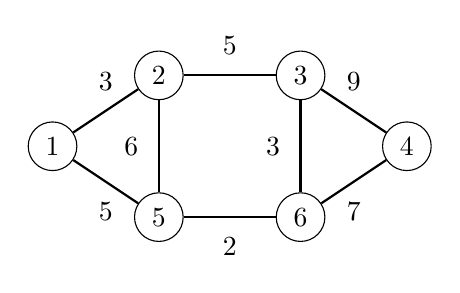
\begin{tikzpicture}[scale=0.9]
\node[draw, circle] (1) at (1.5,2) {$1$};
\node[draw, circle] (2) at (3,3) {$2$};
\node[draw, circle] (3) at (5,3) {$3$};
\node[draw, circle] (4) at (6.5,2) {$4$};
\node[draw, circle] (5) at (3,1) {$5$};
\node[draw, circle] (6) at (5,1) {$6$};
\path[draw,thick,-] (1) -- node[font=\small,label=above:3] {} (2);
\path[draw,thick,-] (2) -- node[font=\small,label=above:5] {} (3);
\path[draw,thick,-] (3) -- node[font=\small,label=above:9] {} (4);
\path[draw,thick,-] (1) -- node[font=\small,label=below:5] {} (5);
\path[draw,thick,-] (5) -- node[font=\small,label=below:2] {} (6);
\path[draw,thick,-] (6) -- node[font=\small,label=below:7] {} (4);
\path[draw,thick,-] (2) -- node[font=\small,label=left:6] {} (5);
\path[draw,thick,-] (3) -- node[font=\small,label=left:3] {} (6);
\end{tikzpicture}
\end{center}
One spanning tree for the graph is as follows:
\begin{center}
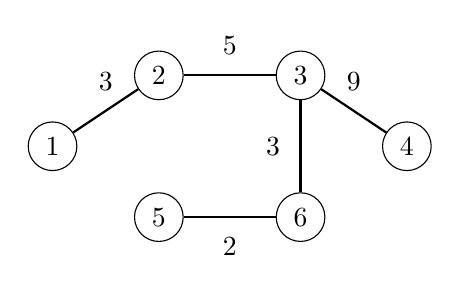
\begin{tikzpicture}[scale=0.9]
\node[draw, circle] (1) at (1.5,2) {$1$};
\node[draw, circle] (2) at (3,3) {$2$};
\node[draw, circle] (3) at (5,3) {$3$};
\node[draw, circle] (4) at (6.5,2) {$4$};
\node[draw, circle] (5) at (3,1) {$5$};
\node[draw, circle] (6) at (5,1) {$6$};
\path[draw,thick,-] (1) -- node[font=\small,label=above:3] {} (2);
\path[draw,thick,-] (2) -- node[font=\small,label=above:5] {} (3);
\path[draw,thick,-] (3) -- node[font=\small,label=above:9] {} (4);
\path[draw,thick,-] (5) -- node[font=\small,label=below:2] {} (6);
\path[draw,thick,-] (3) -- node[font=\small,label=left:3] {} (6);
\end{tikzpicture}
\end{center}

The weight of a spanning tree is the sum of its edge weights.
For example, the weight of the above spanning tree is
$3+5+9+3+2=22$.

\index{minimum spanning tree}

A \key{minimum spanning tree}
is a spanning tree whose weight is as small as possible.
The weight of a minimum spanning tree for the example graph
is 20, and such a tree can be constructed as follows:

\begin{center}
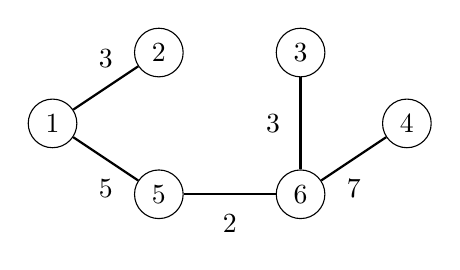
\begin{tikzpicture}[scale=0.9]
\node[draw, circle] (1) at (1.5,2) {$1$};
\node[draw, circle] (2) at (3,3) {$2$};
\node[draw, circle] (3) at (5,3) {$3$};
\node[draw, circle] (4) at (6.5,2) {$4$};
\node[draw, circle] (5) at (3,1) {$5$};
\node[draw, circle] (6) at (5,1) {$6$};

\path[draw,thick,-] (1) -- node[font=\small,label=above:3] {} (2);
\path[draw,thick,-] (1) -- node[font=\small,label=below:5] {} (5);
\path[draw,thick,-] (5) -- node[font=\small,label=below:2] {} (6);
\path[draw,thick,-] (6) -- node[font=\small,label=below:7] {} (4);
\path[draw,thick,-] (3) -- node[font=\small,label=left:3] {} (6);
\end{tikzpicture}
\end{center}

\index{maximum spanning tree}

In a similar way, a \key{maximum spanning tree}
is a spanning tree whose weight is as large as possible.
The weight of a maximum spanning tree for the
example graph is 32:

\begin{center}
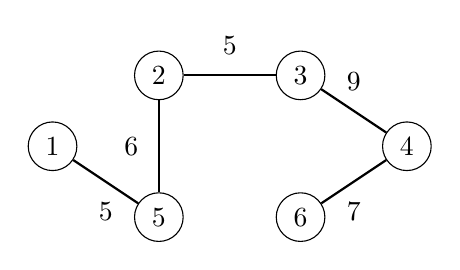
\begin{tikzpicture}[scale=0.9]
\node[draw, circle] (1) at (1.5,2) {$1$};
\node[draw, circle] (2) at (3,3) {$2$};
\node[draw, circle] (3) at (5,3) {$3$};
\node[draw, circle] (4) at (6.5,2) {$4$};
\node[draw, circle] (5) at (3,1) {$5$};
\node[draw, circle] (6) at (5,1) {$6$};
\path[draw,thick,-] (2) -- node[font=\small,label=above:5] {} (3);
\path[draw,thick,-] (3) -- node[font=\small,label=above:9] {} (4);
\path[draw,thick,-] (1) -- node[font=\small,label=below:5] {} (5);
\path[draw,thick,-] (6) -- node[font=\small,label=below:7] {} (4);
\path[draw,thick,-] (2) -- node[font=\small,label=left:6] {} (5);
\end{tikzpicture}
\end{center}

Note that a graph may have several
minimum and maximum spanning trees,
so the trees are not unique.

It turns out that several greedy methods
can be used to construct minimum and maximum
spanning trees.
In this chapter, we discuss two algorithms
that process
the edges of the graph ordered by their weights.
We focus on finding minimum spanning trees,
but the same algorithms can find
maximum spanning trees by processing the edges in reverse order.

\section{Kruskal's algorithm}

\index{Kruskal's algorithm}

In \key{Kruskal's algorithm}\footnote{The algorithm was published in 1956
by J. B. Kruskal \cite{kru56}.}, the initial spanning tree
only contains the nodes of the graph
and does not contain any edges.
Then the algorithm goes through the edges
ordered by their weights, and always adds an edge
to the tree if it does not create a cycle.

The algorithm maintains the components
of the tree.
Initially, each node of the graph
belongs to a separate component.
Always when an edge is added to the tree,
two components are joined.
Finally, all nodes belong to the same component,
and a minimum spanning tree has been found.

\subsubsection{Example}

\begin{samepage}
Let us consider how Kruskal's algorithm processes the
following graph:
\begin{center}
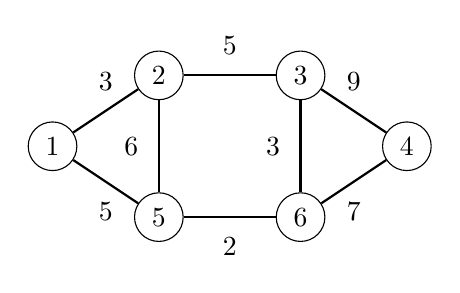
\begin{tikzpicture}[scale=0.9]
\node[draw, circle] (1) at (1.5,2) {$1$};
\node[draw, circle] (2) at (3,3) {$2$};
\node[draw, circle] (3) at (5,3) {$3$};
\node[draw, circle] (4) at (6.5,2) {$4$};
\node[draw, circle] (5) at (3,1) {$5$};
\node[draw, circle] (6) at (5,1) {$6$};
\path[draw,thick,-] (1) -- node[font=\small,label=above:3] {} (2);
\path[draw,thick,-] (2) -- node[font=\small,label=above:5] {} (3);
\path[draw,thick,-] (3) -- node[font=\small,label=above:9] {} (4);
\path[draw,thick,-] (1) -- node[font=\small,label=below:5] {} (5);
\path[draw,thick,-] (5) -- node[font=\small,label=below:2] {} (6);
\path[draw,thick,-] (6) -- node[font=\small,label=below:7] {} (4);
\path[draw,thick,-] (2) -- node[font=\small,label=left:6] {} (5);
\path[draw,thick,-] (3) -- node[font=\small,label=left:3] {} (6);
\end{tikzpicture}
\end{center}
\end{samepage}

\begin{samepage}
The first step of the algorithm is to sort the
edges in increasing order of their weights.
The result is the following list:

\begin{tabular}{ll}
\\
edge & weight \\
\hline
5--6 & 2 \\
1--2 & 3 \\
3--6 & 3 \\
1--5 & 5 \\
2--3 & 5 \\
2--5 & 6 \\
4--6 & 7 \\
3--4 & 9 \\
\\
\end{tabular}
\end{samepage}

After this, the algorithm goes through the list
and adds each edge to the tree if it joins
two separate components.

Initially, each node is in its own component:

\begin{center}
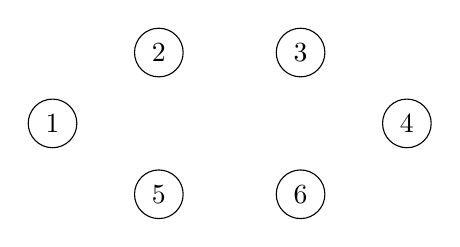
\begin{tikzpicture}[scale=0.9]
\node[draw, circle] (1) at (1.5,2) {$1$};
\node[draw, circle] (2) at (3,3) {$2$};
\node[draw, circle] (3) at (5,3) {$3$};
\node[draw, circle] (4) at (6.5,2) {$4$};
\node[draw, circle] (5) at (3,1) {$5$};
\node[draw, circle] (6) at (5,1) {$6$};
%\path[draw,thick,-] (1) -- node[font=\small,label=above:3] {} (2);
%\path[draw,thick,-] (2) -- node[font=\small,label=above:5] {} (3);
%\path[draw,thick,-] (3) -- node[font=\small,label=above:9] {} (4);
%\path[draw,thick,-] (1) -- node[font=\small,label=below:5] {} (5);
%\path[draw,thick,-] (5) -- node[font=\small,label=below:2] {} (6);
%\path[draw,thick,-] (6) -- node[font=\small,label=below:7] {} (4);
%\path[draw,thick,-] (2) -- node[font=\small,label=left:6] {} (5);
%\path[draw,thick,-] (3) -- node[font=\small,label=left:3] {} (6);
\end{tikzpicture}
\end{center}
The first edge to be added to the tree is
the edge 5--6 that creates a component $\{5,6\}$
by joining the components $\{5\}$ and $\{6\}$:

\begin{center}
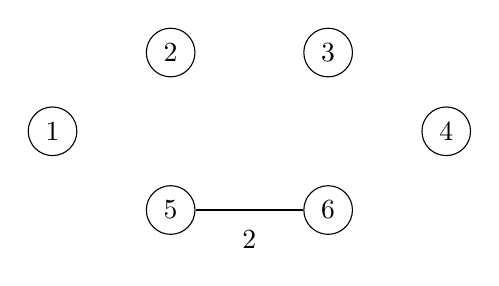
\begin{tikzpicture}
\node[draw, circle] (1) at (1.5,2) {$1$};
\node[draw, circle] (2) at (3,3) {$2$};
\node[draw, circle] (3) at (5,3) {$3$};
\node[draw, circle] (4) at (6.5,2) {$4$};
\node[draw, circle] (5) at (3,1) {$5$};
\node[draw, circle] (6) at (5,1) {$6$};

%\path[draw,thick,-] (1) -- node[font=\small,label=above:3] {} (2);
%\path[draw,thick,-] (2) -- node[font=\small,label=above:5] {} (3);
%\path[draw,thick,-] (3) -- node[font=\small,label=above:9] {} (4);
%\path[draw,thick,-] (1) -- node[font=\small,label=below:5] {} (5);
\path[draw,thick,-] (5) -- node[font=\small,label=below:2] {} (6);
%\path[draw,thick,-] (6) -- node[font=\small,label=below:7] {} (4);
%\path[draw,thick,-] (2) -- node[font=\small,label=left:6] {} (5);
%\path[draw,thick,-] (3) -- node[font=\small,label=left:3] {} (6);
\end{tikzpicture}
\end{center}
After this, the edges 1--2, 3--6 and 1--5 are added in a similar way:

\begin{center}
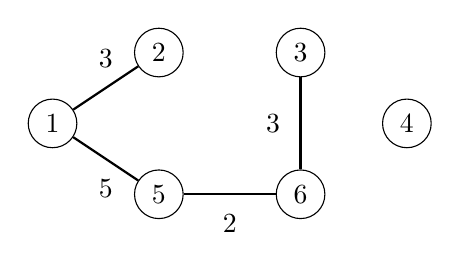
\begin{tikzpicture}[scale=0.9]
\node[draw, circle] (1) at (1.5,2) {$1$};
\node[draw, circle] (2) at (3,3) {$2$};
\node[draw, circle] (3) at (5,3) {$3$};
\node[draw, circle] (4) at (6.5,2) {$4$};
\node[draw, circle] (5) at (3,1) {$5$};
\node[draw, circle] (6) at (5,1) {$6$};

\path[draw,thick,-] (1) -- node[font=\small,label=above:3] {} (2);
%\path[draw,thick,-] (2) -- node[font=\small,label=above:5] {} (3);
%\path[draw,thick,-] (3) -- node[font=\small,label=above:9] {} (4);
\path[draw,thick,-] (1) -- node[font=\small,label=below:5] {} (5);
\path[draw,thick,-] (5) -- node[font=\small,label=below:2] {} (6);
%\path[draw,thick,-] (6) -- node[font=\small,label=below:7] {} (4);
%\path[draw,thick,-] (2) -- node[font=\small,label=left:6] {} (5);
\path[draw,thick,-] (3) -- node[font=\small,label=left:3] {} (6);
\end{tikzpicture}
\end{center}

After those steps, most components have been joined
and there are two components in the tree:
$\{1,2,3,5,6\}$ and $\{4\}$.

The next edge in the list is the edge 2--3,
but it will not be included in the tree, because
nodes 2 and 3 are already in the same component.
For the same reason, the edge 2--5 will not be included in the tree.

\begin{samepage}
Finally, the edge 4--6 will be included in the tree:

\begin{center}
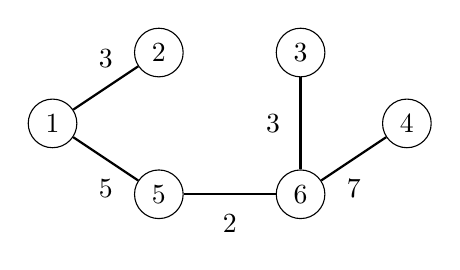
\begin{tikzpicture}[scale=0.9]
\node[draw, circle] (1) at (1.5,2) {$1$};
\node[draw, circle] (2) at (3,3) {$2$};
\node[draw, circle] (3) at (5,3) {$3$};
\node[draw, circle] (4) at (6.5,2) {$4$};
\node[draw, circle] (5) at (3,1) {$5$};
\node[draw, circle] (6) at (5,1) {$6$};

\path[draw,thick,-] (1) -- node[font=\small,label=above:3] {} (2);
%\path[draw,thick,-] (2) -- node[font=\small,label=above:5] {} (3);
%\path[draw,thick,-] (3) -- node[font=\small,label=above:9] {} (4);
\path[draw,thick,-] (1) -- node[font=\small,label=below:5] {} (5);
\path[draw,thick,-] (5) -- node[font=\small,label=below:2] {} (6);
\path[draw,thick,-] (6) -- node[font=\small,label=below:7] {} (4);
%\path[draw,thick,-] (2) -- node[font=\small,label=left:6] {} (5);
\path[draw,thick,-] (3) -- node[font=\small,label=left:3] {} (6);
\end{tikzpicture}
\end{center}
\end{samepage}

After this, the algorithm will not add any
new edges, because the graph is connected
and there is a path between any two nodes.
The resulting graph is a minimum spanning tree
with weight $2+3+3+5+7=20$.

\subsubsection{Why does this work?}

It is a good question why Kruskal's algorithm works.
Why does the greedy strategy guarantee that we
will find a minimum spanning tree?

Let us see what happens if the minimum weight edge of
the graph is \emph{not} included in the spanning tree.
For example, suppose that a spanning tree
for the previous graph would not contain the
minimum weight edge 5--6.
We do not know the exact structure of such a spanning tree,
but in any case it has to contain some edges.
Assume that the tree would be as follows:

\begin{center}
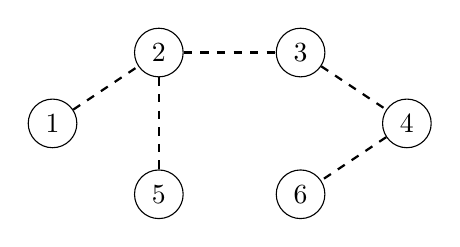
\begin{tikzpicture}[scale=0.9]
\node[draw, circle] (1) at (1.5,2) {$1$};
\node[draw, circle] (2) at (3,3) {$2$};
\node[draw, circle] (3) at (5,3) {$3$};
\node[draw, circle] (4) at (6.5,2) {$4$};
\node[draw, circle] (5) at (3,1) {$5$};
\node[draw, circle] (6) at (5,1) {$6$};

\path[draw,thick,-,dashed] (1) -- (2);
\path[draw,thick,-,dashed] (2) -- (5);
\path[draw,thick,-,dashed] (2) -- (3);
\path[draw,thick,-,dashed] (3) -- (4);
\path[draw,thick,-,dashed] (4) -- (6);
\end{tikzpicture}
\end{center}

However, it is not possible that the above tree
would be a minimum spanning tree for the graph.
The reason for this is that we can remove an edge
from the tree and replace it with the minimum weight edge 5--6.
This produces a spanning tree whose weight is
\emph{smaller}:

\begin{center}
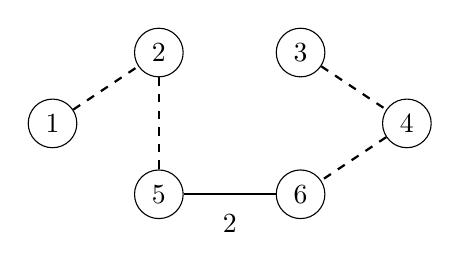
\begin{tikzpicture}[scale=0.9]
\node[draw, circle] (1) at (1.5,2) {$1$};
\node[draw, circle] (2) at (3,3) {$2$};
\node[draw, circle] (3) at (5,3) {$3$};
\node[draw, circle] (4) at (6.5,2) {$4$};
\node[draw, circle] (5) at (3,1) {$5$};
\node[draw, circle] (6) at (5,1) {$6$};

\path[draw,thick,-,dashed] (1) -- (2);
\path[draw,thick,-,dashed] (2) -- (5);
\path[draw,thick,-,dashed] (3) -- (4);
\path[draw,thick,-,dashed] (4) -- (6);
\path[draw,thick,-] (5) -- node[font=\small,label=below:2] {} (6);
\end{tikzpicture}
\end{center}

For this reason, it is always optimal
to include the minimum weight edge
in the tree to produce a minimum spanning tree.
Using a similar argument, we can show that it
is also optimal to add the next edge in weight order
to the tree, and so on.
Hence, Kruskal's algorithm works correctly and
always produces a minimum spanning tree.

\subsubsection{Implementation}

When implementing Kruskal's algorithm,
it is convenient to use
the edge list representation of the graph.
The first phase of the algorithm sorts the
edges in the list in $O(m \log m)$ time.
After this, the second phase of the algorithm
builds the minimum spanning tree as follows:

\begin{lstlisting}
for (...) {
  if (!same(a,b)) unite(a,b);
}
\end{lstlisting}

The loop goes through the edges in the list
and always processes an edge $a$--$b$
where $a$ and $b$ are two nodes.
Two functions are needed:
the function \texttt{same} determines
if $a$ and $b$ are in the same component,
and the function \texttt{unite}
joins the components that contain $a$ and $b$.

The problem is how to efficiently implement
the functions \texttt{same} and \texttt{unite}.
One possibility is to implement the function
\texttt{same} as a graph traversal and check if
we can get from node $a$ to node $b$.
However, the time complexity of such a function
would be $O(n+m)$
and the resulting algorithm would be slow,
because the function \texttt{same} will be called for each edge in the graph.

We will solve the problem using a union-find structure
that implements both functions in $O(\log n)$ time.
Thus, the time complexity of Kruskal's algorithm
will be $O(m \log n)$ after sorting the edge list.

\section{Union-find structure}

\index{union-find structure}

A \key{union-find structure} maintains
a collection of sets.
The sets are disjoint, so no element
belongs to more than one set.
Two $O(\log n)$ time operations are supported:
the \texttt{unite} operation joins two sets,
and the \texttt{find} operation finds the representative
of the set that contains a given element\footnote{The structure presented here
was introduced in 1971 by J. D. Hopcroft and J. D. Ullman \cite{hop71}.
Later, in 1975, R. E. Tarjan studied a more sophisticated variant
of the structure \cite{tar75} that is discussed in many algorithm
textbooks nowadays.}.

\subsubsection{Structure}

In a union-find structure, one element in each set
is the representative of the set,
and there is a chain from any other element of the
set to the representative.
For example, assume that the sets are
$\{1,4,7\}$, $\{5\}$ and $\{2,3,6,8\}$:
\begin{center}
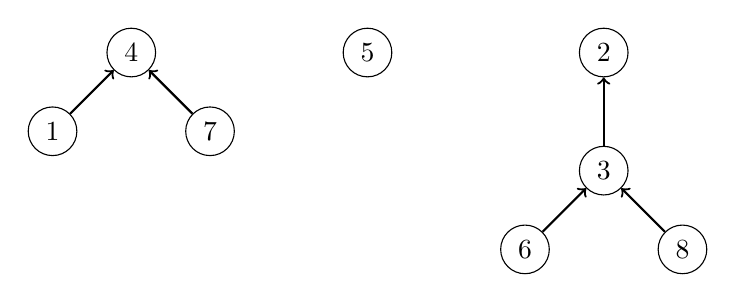
\begin{tikzpicture}
\node[draw, circle] (1) at (0,-1) {$1$};
\node[draw, circle] (2) at (7,0) {$2$};
\node[draw, circle] (3) at (7,-1.5) {$3$};
\node[draw, circle] (4) at (1,0) {$4$};
\node[draw, circle] (5) at (4,0) {$5$};
\node[draw, circle] (6) at (6,-2.5) {$6$};
\node[draw, circle] (7) at (2,-1) {$7$};
\node[draw, circle] (8) at (8,-2.5) {$8$};

\path[draw,thick,->] (1) -- (4);
\path[draw,thick,->] (7) -- (4);

\path[draw,thick,->] (3) -- (2);
\path[draw,thick,->] (6) -- (3);
\path[draw,thick,->] (8) -- (3);

\end{tikzpicture}
\end{center}
In this case the representatives
of the sets are 4, 5 and 2.
We can find the representative of any element
by following the chain that begins at the element.
For example, the element 2 is the representative
for the element 6, because
we follow the chain $6 \rightarrow 3 \rightarrow 2$.
Two elements belong to the same set exactly when
their representatives are the same.

Two sets can be joined by connecting the
representative of one set to the
representative of the other set.
For example, the sets
$\{1,4,7\}$ and $\{2,3,6,8\}$
can be joined as follows:
\begin{center}
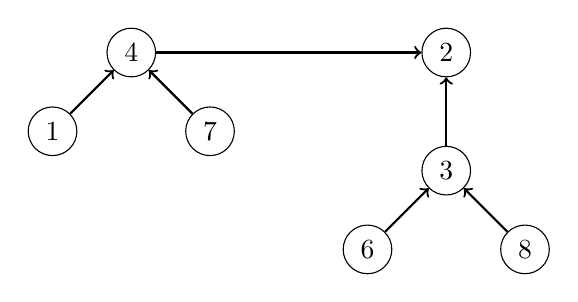
\begin{tikzpicture}
\node[draw, circle] (1) at (2,-1) {$1$};
\node[draw, circle] (2) at (7,0) {$2$};
\node[draw, circle] (3) at (7,-1.5) {$3$};
\node[draw, circle] (4) at (3,0) {$4$};
\node[draw, circle] (6) at (6,-2.5) {$6$};
\node[draw, circle] (7) at (4,-1) {$7$};
\node[draw, circle] (8) at (8,-2.5) {$8$};

\path[draw,thick,->] (1) -- (4);
\path[draw,thick,->] (7) -- (4);

\path[draw,thick,->] (3) -- (2);
\path[draw,thick,->] (6) -- (3);
\path[draw,thick,->] (8) -- (3);

\path[draw,thick,->] (4) -- (2);
\end{tikzpicture}
\end{center}

The resulting set contains the elements
$\{1,2,3,4,6,7,8\}$.
From this on, the element 2 is the representative
for the entire set and the old representative 4
points to the element 2.

The efficiency of the union-find structure depends on
how the sets are joined.
It turns out that we can follow a simple strategy:
always connect the representative of the
\emph{smaller} set to the representative of the \emph{larger} set
(or if the sets are of equal size,
we can make an arbitrary choice).
Using this strategy, the length of any chain
will be $O(\log n)$, so we can
find the representative of any element
efficiently by following the corresponding chain.

\subsubsection{Implementation}

The union-find structure can be implemented
using arrays.
In the following implementation,
the array \texttt{link} contains for each element
the next element
in the chain or the element itself if it is
a representative,
and the array \texttt{size} indicates for each representative
the size of the corresponding set.

Initially, each element belongs to a separate set:
\begin{lstlisting}
for (int i = 1; i <= n; i++) link[i] = i;
for (int i = 1; i <= n; i++) size[i] = 1;
\end{lstlisting}

The function \texttt{find} returns
the representative for an element $x$.
The representative can be found by following
the chain that begins at $x$.

\begin{lstlisting}
int find(int x) {
    while (x != link[x]) x = link[x];
    return x;
}
\end{lstlisting}

The function \texttt{same} checks
whether elements $a$ and $b$ belong to the same set.
This can easily be done by using the
function \texttt{find}:

\begin{lstlisting}
bool same(int a, int b) {
    return find(a) == find(b);
}
\end{lstlisting}

\begin{samepage}
The function \texttt{unite} joins the sets
that contain elements $a$ and $b$
(the elements have to be in different sets).
The function first finds the representatives
of the sets and then connects the smaller
set to the larger set.

\begin{lstlisting}
void unite(int a, int b) {
    a = find(a);
    b = find(b);
    if (size[a] < size[b]) swap(a,b);
    size[a] += size[b];
    link[b] = a;
}
\end{lstlisting}
\end{samepage}

The time complexity of the function \texttt{find}
is $O(\log n)$ assuming that the length of each
chain is $O(\log n)$.
In this case, the functions \texttt{same} and \texttt{unite}
also work in $O(\log n)$ time.
The function \texttt{unite} makes sure that the
length of each chain is $O(\log n)$ by connecting
the smaller set to the larger set.

\section{Prim's algorithm}

\index{Prim's algorithm}

\key{Prim's algorithm}\footnote{The algorithm is
named after R. C. Prim who published it in 1957 \cite{pri57}.
However, the same algorithm was discovered already in 1930
by V. Jarník.} is an alternative method
for finding a minimum spanning tree.
The algorithm first adds an arbitrary node
to the tree.
After this, the algorithm always chooses
a minimum-weight edge that
adds a new node to the tree.
Finally, all nodes have been added to the tree
and a minimum spanning tree has been found.

Prim's algorithm resembles Dijkstra's algorithm.
The difference is that Dijkstra's algorithm always
selects an edge whose distance from the starting
node is minimum, but Prim's algorithm simply selects
the minimum weight edge that adds a new node to the tree.

\subsubsection{Example}

Let us consider how Prim's algorithm works
in the following graph:

\begin{center}
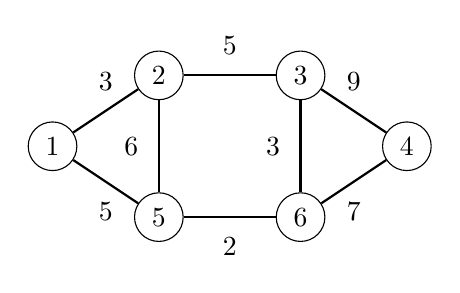
\begin{tikzpicture}[scale=0.9]
\node[draw, circle] (1) at (1.5,2) {$1$};
\node[draw, circle] (2) at (3,3) {$2$};
\node[draw, circle] (3) at (5,3) {$3$};
\node[draw, circle] (4) at (6.5,2) {$4$};
\node[draw, circle] (5) at (3,1) {$5$};
\node[draw, circle] (6) at (5,1) {$6$};
\path[draw,thick,-] (1) -- node[font=\small,label=above:3] {} (2);
\path[draw,thick,-] (2) -- node[font=\small,label=above:5] {} (3);
\path[draw,thick,-] (3) -- node[font=\small,label=above:9] {} (4);
\path[draw,thick,-] (1) -- node[font=\small,label=below:5] {} (5);
\path[draw,thick,-] (5) -- node[font=\small,label=below:2] {} (6);
\path[draw,thick,-] (6) -- node[font=\small,label=below:7] {} (4);
\path[draw,thick,-] (2) -- node[font=\small,label=left:6] {} (5);
\path[draw,thick,-] (3) -- node[font=\small,label=left:3] {} (6);

%\path[draw=red,thick,-,line width=2pt] (5) -- (6);
\end{tikzpicture}
\end{center}
Initially, there are no edges between the nodes:
\begin{center}
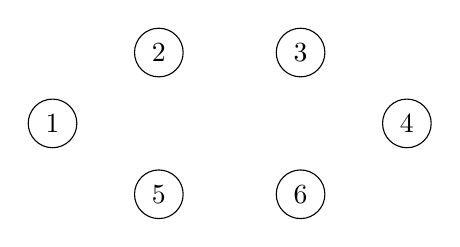
\begin{tikzpicture}[scale=0.9]
\node[draw, circle] (1) at (1.5,2) {$1$};
\node[draw, circle] (2) at (3,3) {$2$};
\node[draw, circle] (3) at (5,3) {$3$};
\node[draw, circle] (4) at (6.5,2) {$4$};
\node[draw, circle] (5) at (3,1) {$5$};
\node[draw, circle] (6) at (5,1) {$6$};
%\path[draw,thick,-] (1) -- node[font=\small,label=above:3] {} (2);
%\path[draw,thick,-] (2) -- node[font=\small,label=above:5] {} (3);
%\path[draw,thick,-] (3) -- node[font=\small,label=above:9] {} (4);
%\path[draw,thick,-] (1) -- node[font=\small,label=below:5] {} (5);
%\path[draw,thick,-] (5) -- node[font=\small,label=below:2] {} (6);
%\path[draw,thick,-] (6) -- node[font=\small,label=below:7] {} (4);
%\path[draw,thick,-] (2) -- node[font=\small,label=left:6] {} (5);
%\path[draw,thick,-] (3) -- node[font=\small,label=left:3] {} (6);
\end{tikzpicture}
\end{center}
An arbitrary node can be the starting node,
so let us choose node 1.
First, we add node 2 that is connected by
an edge of weight 3:
\begin{center}
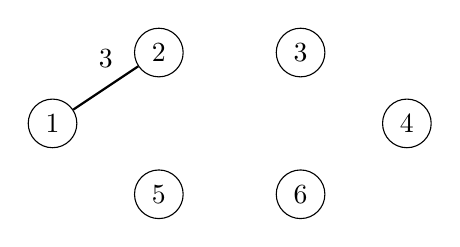
\begin{tikzpicture}[scale=0.9]
\node[draw, circle] (1) at (1.5,2) {$1$};
\node[draw, circle] (2) at (3,3) {$2$};
\node[draw, circle] (3) at (5,3) {$3$};
\node[draw, circle] (4) at (6.5,2) {$4$};
\node[draw, circle] (5) at (3,1) {$5$};
\node[draw, circle] (6) at (5,1) {$6$};
\path[draw,thick,-] (1) -- node[font=\small,label=above:3] {} (2);
%\path[draw,thick,-] (2) -- node[font=\small,label=above:5] {} (3);
%\path[draw,thick,-] (3) -- node[font=\small,label=above:9] {} (4);
%\path[draw,thick,-] (1) -- node[font=\small,label=below:5] {} (5);
%\path[draw,thick,-] (5) -- node[font=\small,label=below:2] {} (6);
%\path[draw,thick,-] (6) -- node[font=\small,label=below:7] {} (4);
%\path[draw,thick,-] (2) -- node[font=\small,label=left:6] {} (5);
%\path[draw,thick,-] (3) -- node[font=\small,label=left:3] {} (6);
\end{tikzpicture}
\end{center}

After this, there are two edges with weight 5,
so we can add either node 3 or node 5 to the tree.
Let us add node 3 first:
\begin{center}
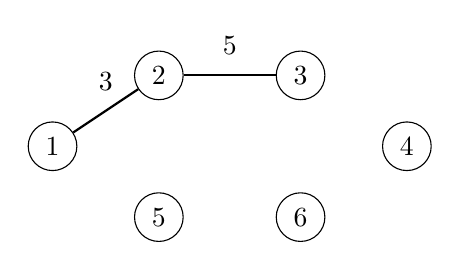
\begin{tikzpicture}[scale=0.9]
\node[draw, circle] (1) at (1.5,2) {$1$};
\node[draw, circle] (2) at (3,3) {$2$};
\node[draw, circle] (3) at (5,3) {$3$};
\node[draw, circle] (4) at (6.5,2) {$4$};
\node[draw, circle] (5) at (3,1) {$5$};
\node[draw, circle] (6) at (5,1) {$6$};
\path[draw,thick,-] (1) -- node[font=\small,label=above:3] {} (2);
\path[draw,thick,-] (2) -- node[font=\small,label=above:5] {} (3);
%\path[draw,thick,-] (3) -- node[font=\small,label=above:9] {} (4);
%\path[draw,thick,-] (1) -- node[font=\small,label=below:5] {} (5);
%\path[draw,thick,-] (5) -- node[font=\small,label=below:2] {} (6);
%\path[draw,thick,-] (6) -- node[font=\small,label=below:7] {} (4);
%\path[draw,thick,-] (2) -- node[font=\small,label=left:6] {} (5);
%\path[draw,thick,-] (3) -- node[font=\small,label=left:3] {} (6);
\end{tikzpicture}
\end{center}

\begin{samepage}
The process continues until all nodes have been included in the tree:
\begin{center}
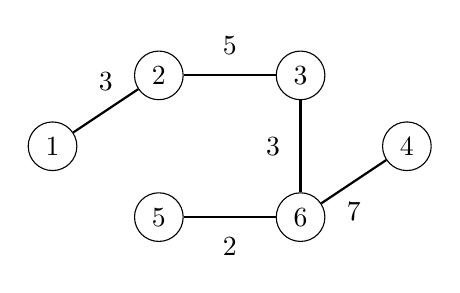
\begin{tikzpicture}[scale=0.9]
\node[draw, circle] (1) at (1.5,2) {$1$};
\node[draw, circle] (2) at (3,3) {$2$};
\node[draw, circle] (3) at (5,3) {$3$};
\node[draw, circle] (4) at (6.5,2) {$4$};
\node[draw, circle] (5) at (3,1) {$5$};
\node[draw, circle] (6) at (5,1) {$6$};
\path[draw,thick,-] (1) -- node[font=\small,label=above:3] {} (2);
\path[draw,thick,-] (2) -- node[font=\small,label=above:5] {} (3);
%\path[draw,thick,-] (3) -- node[font=\small,label=above:9] {} (4);
%\path[draw,thick,-] (1) -- node[font=\small,label=below:5] {} (5);
\path[draw,thick,-] (5) -- node[font=\small,label=below:2] {} (6);
\path[draw,thick,-] (6) -- node[font=\small,label=below:7] {} (4);
%\path[draw,thick,-] (2) -- node[font=\small,label=left:6] {} (5);
\path[draw,thick,-] (3) -- node[font=\small,label=left:3] {} (6);
\end{tikzpicture}
\end{center}
\end{samepage}

\subsubsection{Implementation}

Like Dijkstra's algorithm, Prim's algorithm can be
efficiently implemented using a priority queue.
The priority queue should contain all nodes
that can be connected to the current component using
a single edge, in increasing order of the weights
of the corresponding edges.

The time complexity of Prim's algorithm is
$O(n + m \log m)$ that equals the time complexity
of Dijkstra's algorithm.
In practice, Prim's and Kruskal's algorithms
are both efficient, and the choice of the algorithm
is a matter of taste.
Still, most competitive programmers use Kruskal's algorithm.